\documentclass{beamer}

% \usepackage{amsmath,amssymb,graphicx,hyperref}
% \usepackage{multirow}

\usepackage{graphicx}
\usepackage{amsmath}
\usepackage{amssymb}
% \usepackage{enumitem}
\usepackage{color}
\usepackage{hyperref}
\usepackage{caption}
\usepackage[absolute,overlay]{textpos}
% \usepackage{tikz}
% \usepackage{makecell}
\usepackage{fontawesome}

% \usetheme{Madrid}
% \usecolortheme{seahorse}
\usetheme{AnnArbor}
\usecolortheme{rose}
\usefonttheme{professionalfonts}

\setbeamercolor{title page header}{fg=,bg=}  % 使用主题默认前景色
\setbeamercolor{frametitle}{bg=}  

\title{Split Quaternion Matrices: An Algorithm for QR Decomposition}
\author[Liu QQ]{Qianqian Liu}
\institute[MUST]{Macau University of Science and Technology \\ University of Manitoba}
\date{\today}

\logo{
    
\includegraphics[height=1cm]{images/must-logo.png}
}


\begin{document}

% Title Page
\begin{frame}
  \titlepage
\end{frame}

\logo{%
    \begin{textblock*}{5cm}(11.5cm,0.4cm) % {宽度}(水平位置,垂直位置)
        
\includegraphics[height=0.95cm]{images/must-logo.png}
    \end{textblock*}
}

% Section 1: Introduction
\section{1. Introduction to Split Quaternions}
\begin{frame}{Outline}
  \tableofcontents[sectionstyle=show/shaded, subsectionstyle=show/show/shaded]
\end{frame}

\begin{frame}{1.1 What is Split Quaternion Algebra?}
  \begin{exampleblock}{Definition (Cockle, 1849)}
    Split quaternion algebra over $\mathbb{R}$:
    \[
    \mathbb{H}_{s}=\left\{a_{0}+a_{1}i+a_{2}j+a_{3}k \mid 
    \begin{aligned}
    &i^2=-1,\ j^2=k^2=1, \\
    &ijk=1,\ a_0,a_1,a_2,a_3\in\mathbb{R}
    \end{aligned}\right\}
    \]
  \end{exampleblock}
  \vspace{0em}
  
  \begin{columns}[T]
    \column{0.45\textwidth}
    \textbf{Key Properties}
    \begin{itemize}
        \item[$\bullet$] four-dimensional non-commutative algebra
        \item[$\bullet$] Contains \textbf{zero divisors} (not a Euclidean space)
        \item[$\bullet$] Applications: Quantum mechanics, electromagnetism, signal processing
    \end{itemize}
      
    % \end{block}
    
    \column{0.5\textwidth}
    \textbf{Research Gap}
    %   Existing work covers:
    \begin{itemize}
        \item[$\bullet$] Eigenvalue problems (Jiang et al., 2018a)
        \item[$\bullet$] LDU/SVD decomposition (Wang et al., 2021, 2024)
        \item[$\bullet$] Matrix equations (Si et al., 2024)
        % \vspace{0.5cm}
        \item[$\bullet$] Missing: \textbf{QR decomposition theory \& algorithms}
    \end{itemize}
    % \end{block}
  \end{columns}
\end{frame}

\begin{frame}{1.2 Challenge for Traditional QR Decomposition}
  Traditional QR relies on:
  \begin{itemize}
    \item Givens rotations
    \item Householder reflections
  \end{itemize}
  
  \begin{alertblock}{Critical Limitation}
    $\mathbb{H}_s$ is not a Euclidean space (due to zero divisors). Thus:
  \begin{itemize}
    \item Givens/Householder transformations fail for split quaternion vectors 
    \item Non-commutativity of multiplication adds further complexity
  \end{itemize}
\end{alertblock}
  
  \begin{block}{Our Solution}
   \begin{itemize}
    \item Use \textbf{real representation} of split quaternion matrices to convert the problem into real matrix decomposition!
    \item propose a novel and efficient algorithm for its computation
   \end{itemize}
  \end{block}
\end{frame}

% Section 2: Preliminaries
\section{2. Preliminaries: Real Representation}
\begin{frame}{Outline}
  \tableofcontents[sectionstyle=show/shaded, subsectionstyle=show/show/shaded]
\end{frame}

\begin{frame}{2.1 Real Representation of Split Quaternion Matrices}
  Let $A = A_0 + A_1i + A_2j + A_3k \in \mathbb{H}_s^{m \times n}$ ($A_i \in \mathbb{R}^{m \times n}$).
  
  \begin{block}{Compact Real Representation (Wang et al., 2024)}
    \[
    A^\sigma = \begin{bmatrix}
    A_0 + A_2 & -A_1 + A_3 \\
    A_1 + A_3 & A_0 - A_2
    \end{bmatrix} \in \mathbb{R}^{2m \times 2n}
    \]
    Advantage: Lower dimension ($2m \times 2n$) vs. $4m \times 4n$ (Liu \& Zhang, 2019)
  \end{block}
  
  \begin{block}{Key Isomorphism Properties}
    For $A,B \in \mathbb{H}_s^{m \times n}$, $C \in \mathbb{H}_s^{n \times p}$, $a \in \mathbb{R}$:
    \[
    (A+B)^\sigma = A^\sigma+B^\sigma,\ (AC)^\sigma = A^\sigma C^\sigma,\ (aA)^\sigma = aA^\sigma,\ (A^H)^\sigma = (A^\sigma)^T
    \]
  \end{block}
\end{frame}

\begin{frame}{2.2 Inverse Mapping \& Unitary Property}
  \begin{block}{From Real Matrix to Split Quaternion Matrix}
    For $B = \begin{bmatrix} B_{11} & B_{12} \\ B_{21} & B_{22} \end{bmatrix} \in \mathbb{R}^{2m \times 2n}$, the corresponding $A \in \mathbb{H}_s^{m \times n}$ is:
    \[
    A = \frac{B_{11}+B_{22}}{2} + \frac{B_{21}-B_{12}}{2}i + \frac{B_{11}-B_{22}}{2}j + \frac{B_{21}+B_{12}}{2}k
    \]
    Satisfies: $A^\sigma = B$ (one-to-one correspondence)
  \end{block}
  
  \begin{block}{Unitary $\leftrightarrow$ Orthogonal}
    A split quaternion matrix $Q$ is \textbf{unitary} ($QQ^H = Q^HQ = I$) if and only if $Q^\sigma$ is \textbf{orthogonal} ($(Q^\sigma)^T Q^\sigma = I$).
  \end{block}
  
  \begin{block}{Frobenius Norm Consistency}
    \[
    \|A\|_F = \frac{1}{\sqrt{2}}\|A^\sigma\|_F = \sqrt{\|A_0\|_F^2 + \|A_1\|_F^2 + \|A_2\|_F^2 + \|A_3\|_F^2}
    \]
  \end{block}
\end{frame}

% Section 3: QR Decomposition
\section{3. QR Decomposition of Split Quaternion Matrices}
\begin{frame}{Outline}
  \tableofcontents[sectionstyle=show/shaded, subsectionstyle=show/show/shaded]
\end{frame}

\begin{frame}{3.1 Core Idea: Two-Step Decomposition}
  Goal: For $A \in \mathbb{H}_s^{m \times n}$, find unitary $Q \in \mathbb{H}_s^{m \times m}$ and upper triangular $R \in \mathbb{H}_s^{m \times n}$ such that $A = QR$.

  \begin{block}{Step 1: Special Real Decomposition}
    Compute $A^\sigma = \tilde{Q} R_4$, where:
   \begin{itemize}
    \item $\tilde{Q} \in \mathbb{R}^{2m \times 2m}$: Orthogonal matrix\\
    \item $R_4 \in \mathbb{R}^{2m \times 2n}$: Block upper triangular:
      \[
      R_4 = \begin{bmatrix} R_{11} & R_{12} \\ R_{21} & R_{22} \end{bmatrix}, \quad R_{11},R_{12},R_{21},R_{22} \in \mathbb{R}^{m \times n} \text{ (upper triangular)}
      \]
   \end{itemize}
  \end{block}
  
  \begin{block}{Step 2: Map Back to Split Quaternions}
    Use inverse mapping (Section 2.2) to construct:
   \begin{itemize}
    \item $Q$ from $\tilde{Q}$ (unitary)
    \item $R$ from $R_4$ (upper triangular)
   \end{itemize}
    Satisfies: $A = QR$
  \end{block}
%   \begin{block}{Step 1: Special Real Decomposition}
%         Construct a special decomposition of the real representation \( A^\sigma \):
%         \[
%         A^\sigma = \widetilde{Q} R_4
%         \]
%         where \( \widetilde{Q} \in \mathbb{R}^{2m \times 2m} \) is orthogonal, and \( R_4 \) is in the form of 
% \begin{equation}\label{r4}
% R_4 = \begin{bmatrix}
%     R_{11} & R_{12} \\
%     R_{21} & R_{22}
% \end{bmatrix} \in \mathbb{R}^{2m \times 2n},
% \end{equation}
% and $R_{11}, R_{12},R_{21},R_{22}$ are all upper triangular matrices of size $m \times n$.
% \end{block}
% \begin{block}{Step 2: Map Back to Split Quaternions}  
%          \textbf{Step 2:} Construct split quaternion matrices \( Q \) (unitary) and \( R \) (upper triangular) such that \( A = QR \).
%  \end{block}
\end{frame}

\begin{frame}{3.2 Permutation Transformations}
  Convert standard real QR's upper triangular $R$ to $R_4$ via row/column permutations.
  
  \begin{block}{Permutation Matrix $P_{2k}$ ($k=m,n$)}
    \[
    P_{2k} = \begin{bmatrix}
    1 & 0 & 0 & \cdots & 0 \\
    0 & 0 & 1 & \cdots & 0 \\
    \vdots & \vdots & \vdots & \ddots & \vdots \\
    0 & 1 & 0 & \cdots & 0 \\
    0 & 0 & 0 & \cdots & 1
    \end{bmatrix}_{2k \times 2k}
    \]
    Swaps even rows/columns with specific odd rows/columns.
  \end{block}
  \end{frame}

  \begin{frame}{3.2 How to Get $R_4$?}
  \begin{block}{Key Relationship}
    \[
    P_{2m} R P_{2n}^T = \begin{bmatrix} R_{11} & R_{12} \\ R_{21} & R_{22} \end{bmatrix} = R_4
    \]
    Where $R$ is the upper triangular matrix from standard real QR.
  \end{block}
  
  \begin{figure}[h]
    \centering
    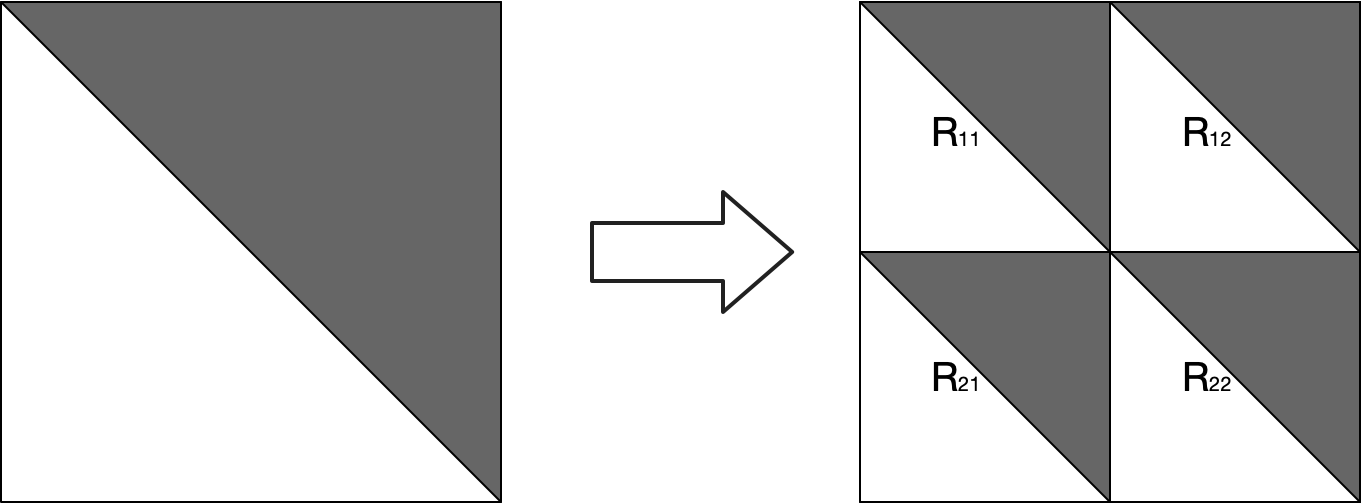
\includegraphics[width=0.6\textwidth]{images/Figure_1.png} % Replace with actual figure
    \caption{From $R$ to $R_4$ via permutations}
  \end{figure}
\end{frame}

\begin{frame}{3.3 Proof of QR Decomposition Existence}
  \begin{block}{Theorem 3.1 (QR Decomposition for $\mathbb{H}_s$)}
    For any $A \in \mathbb{H}_s^{m \times n}$, there exist:\\
    - Unitary $Q \in \mathbb{H}_s^{m \times m}$\\
    - Upper triangular $R \in \mathbb{H}_s^{m \times n}$
    Such that $A = QR$.
  \end{block}
\end{frame}
\begin{frame}{3.3 Proof of QR Decomposition Existence}
%   \begin{proof}[Sketch]
    \begin{enumerate}
    \item Compute standard QR of $P_{2m}^T A^\sigma P_{2n}$:
       \[
       P_{2m}^T A^\sigma P_{2n} = \hat{Q} \hat{R}
       \]
       ($\hat{Q}$ orthogonal, $\hat{R}$ upper triangular)
    \vspace{1em}

    \item Multiply both sides by $P_{2m}$ (left) and $P_{2n}^T$ (right):
       \[
       A^\sigma = P_{2m} \hat{Q} P_{2m}^T \cdot P_{2m} \hat{R} P_{2n}^T = \tilde{Q} R_4
       \]
       ($\tilde{Q} = P_{2m} \hat{Q} P_{2m}^T$ orthogonal, $R_4 = P_{2m} \hat{R} P_{2n}^T$ block upper triangular)
    \vspace{1em}

    \item Map $\tilde{Q} \to Q$ (unitary) and $R_4 \to R$ (upper triangular) via inverse mapping. Then $A^\sigma = Q^\sigma R^\sigma \implies A = QR$.
%   \end{proof}
    \end{enumerate}
\end{frame}

% Section 4: Algorithms
\section{4. Efficient Algorithms}
\begin{frame}{Outline}
  \tableofcontents[sectionstyle=show/shaded, subsectionstyle=show/show/shaded]
\end{frame}

\begin{frame}{4.1 Algorithm 1: Recursive Permutation}
  \begin{block}{Function Permutation(P)}
    Input: $P \in \mathbb{R}^{2s \times 2n}$ (matrix to permute) \\
    Output: Permuted $P \in \mathbb{R}^{2s \times 2n}$
    \begin{enumerate}
      \item If $s=1$, return $P$ (base case)
      \item Compute $s2 = \lfloor s/2 \rfloor$
      \item Swap even rows in upper half with odd rows in lower half:
        \[
        P = \begin{cases} 
        \text{swap}(P, 2i, s+2i-1) & \text{if } s \text{ even} \\
        \text{swap}(P, 2i, s+2i) & \text{if } s \text{ odd}
        \end{cases} \quad (i=1,\dots,s2)
        \]
      \item Partition $P$ into $P_{upper}$ and $P_{lower}$ (add zero rows if $s$ odd)
      \item Recursively permute $P_{upper}$ and $P_{lower}$
      \item Remove zero rows and reconstruct $P$
    \end{enumerate}
  \end{block}
\end{frame}

\begin{frame}{4.2 Algorithm 2: Optimized Permutation (Reduce Cost)}
  Avoids matrix multiplication by direct row/column assignment.
  
  \begin{block}{Function PermutationOpt(A, t)}
    Input: $A \in \mathbb{R}^{2m \times 2n}$, $t \in \{0,1\}$ \\ % 修复:补全集合右括号​
    Output: $B = \begin{cases} P_{2m} A P_{2n}^T & t=0 \\ P_{2m}^T A P_{2n} & t=1 \end{cases}$
    \begin{itemize}
      \item Case $t=0$:
        \begin{enumerate}
          \item Assign odd rows of $A$ to 1st-$m$th rows of $A_{tmp}$; 
                even rows to $(m+1)$th-$2m$th rows
          \item Assign odd columns of $A_{tmp}$ to 1st-$n$th columns of $B$; 
                even columns to $(n+1)$th-$2n$th columns
        \end{enumerate}
      \item Case $t=1$: Reverse the above steps
    \end{itemize}
  \end{block}
\end{frame}

\begin{frame}{4.3 Algorithm 3: Split Quaternion QR Decomposition}
\footnotesize
    Input: $A = A_0 + A_1i + A_2j + A_3k \in \mathbb{H}_s^{m \times n}$ \\
    Output: Unitary $Q$, upper triangular $R$ with $A=QR$
    \begin{enumerate}
      \item Compute real representation:
        \[
        A^\sigma = \begin{bmatrix} A_0+A_2 & -A_1+A_3 \\ A_1+A_3 & A_0-A_2 \end{bmatrix}
        \]
      \item Permute $A^\sigma$: $\hat{A} = \text{PermutationOpt}(A^\sigma, 1)$
      \item Standard real QR: $[\hat{Q}, \hat{R}] = \text{qr}(\hat{A})$
      \item Permute back: $R_4 = \text{PermutationOpt}(\hat{R}, 0)$, $\tilde{Q} = \text{PermutationOpt}(\hat{Q}, 0)$
      \item Construct $Q$ and $R$ via inverse mapping:
        \begin{align*}
        Q &= \frac{Q_{11}+Q_{22}}{2} + \frac{Q_{21}-Q_{12}}{2}i + \frac{Q_{11}-Q_{22}}{2}j + \frac{Q_{21}+Q_{12}}{2}k \\
        R &= \frac{R_{11}+R_{22}}{2} + \frac{R_{21}-R_{12}}{2}i + \frac{R_{11}-R_{22}}{2}j + \frac{R_{21}+R_{12}}{2}k
        \end{align*}
        (where $\tilde{Q} = \begin{bmatrix} Q_{11} & Q_{12} \\ Q_{21} & Q_{22} \end{bmatrix}$, $R_4 = \begin{bmatrix} R_{11} & R_{12} \\ R_{21} & R_{22} \end{bmatrix}$)
    \end{enumerate}
%   \end{block}
\end{frame}

\begin{frame}{4.4 Computational Complexity Analysis}
  For $A \in \mathbb{H}_s^{m \times n}$, total complexity is dominated by real QR:
  
  \begin{columns}[T]
    \column{0.32\textwidth}
    \begin{block}{1. Real Representation}
      $4mn$ flops
    \end{block}
    
    \column{0.25\textwidth}
    \begin{block}{2. Optimized Permutation}
      $8m + 4n$ flops
    \end{block}
    
    \column{0.38\textwidth}
    \begin{block}{3. Real QR Decomposition}
      $16\left(mn^2 - \frac{n^3}{3}\right)$ flops (Householder reflections)
    \end{block}
  \end{columns}
  
  \begin{block}{Total Complexity}
    \[
    \underbrace{4mn}_{\text{Real Rep.}} + \underbrace{8m+4n}_{\text{Permutation}} + \underbrace{16\left(mn^2 - \frac{n^3}{3}\right)}_{\text{Real QR}} \approx 16\left(mn^2 - \frac{n^3}{3}\right)
    \]
  \end{block}
\end{frame}

% Section 5: Numerical Examples
\section{5. Numerical Experiments}
\begin{frame}{Outline}
  \tableofcontents[sectionstyle=show/shaded, subsectionstyle=show/show/shaded]
\end{frame}

\begin{frame}{5.1 Example 4.1: Efficiency \& Accuracy Test}
  \begin{block}{Experiment Setup}
    - Test matrices: $A = A_0 + A_1i + A_2j + A_3k$, $A_i = \text{rand}(m,n)$ ($0 < A_{i,ij} < 1$)\\
    - Sizes: $m,n = 50,100,\dots,1000$\\
    % - Environment: MATLAB 2024a, Intel i7-1185G7, 16GB RAM, Windows 11
    - Metrics: CPU time, relative error $\epsilon = \frac{\|A - QR\|_F}{\|A\|_F}$
  \end{block}
  
  \begin{figure}[h]
    \centering
    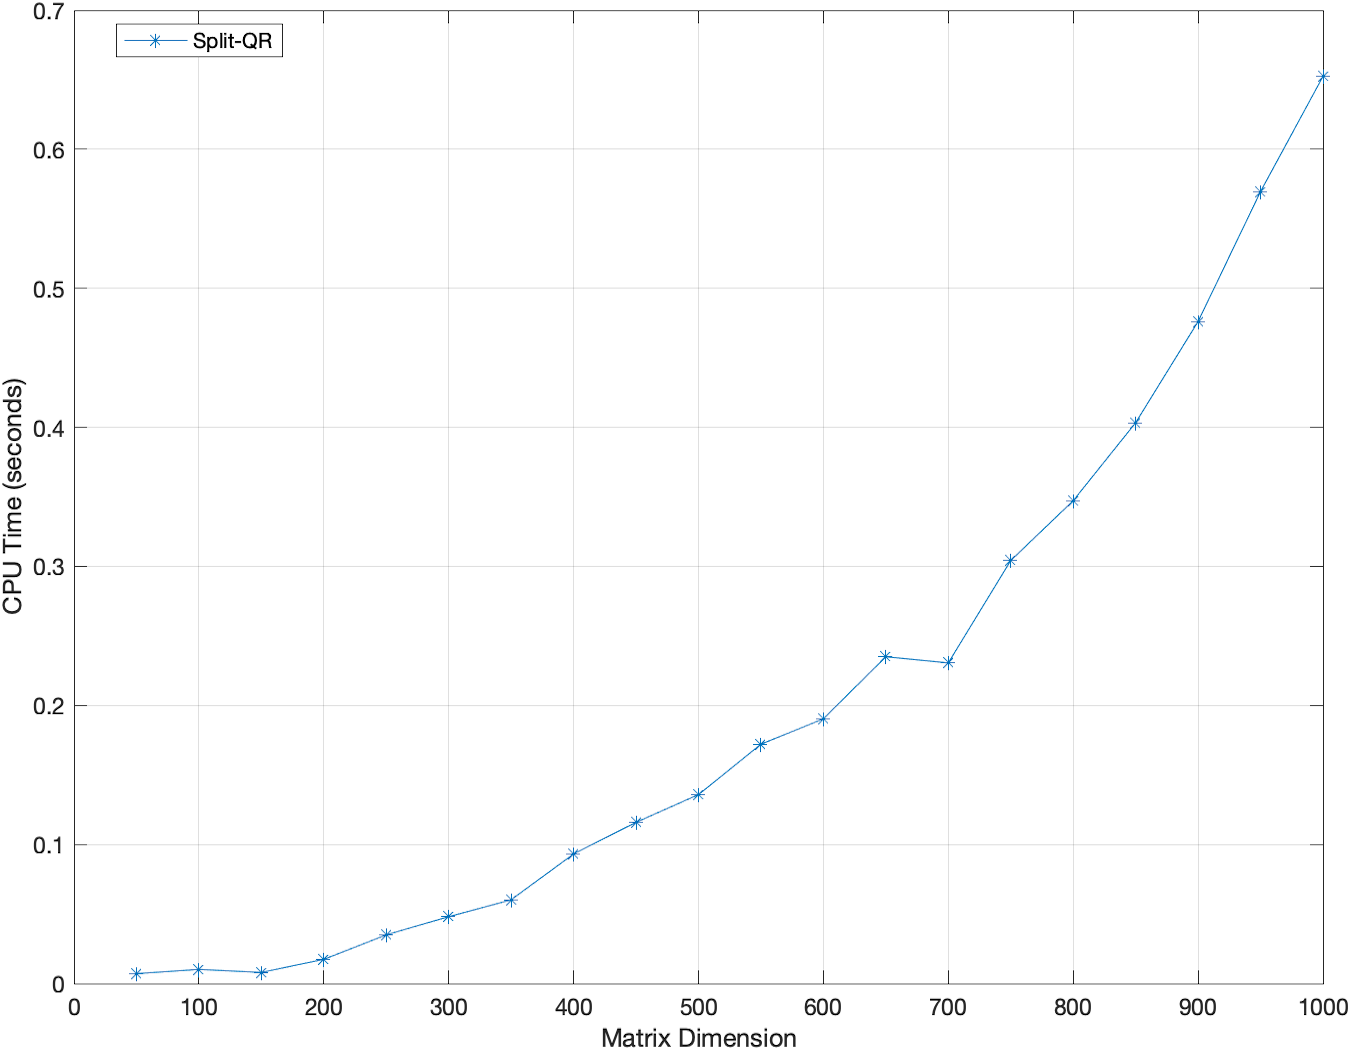
\includegraphics[width=0.45\textwidth]{images/Figure_2.png} % Replace with actual figure
    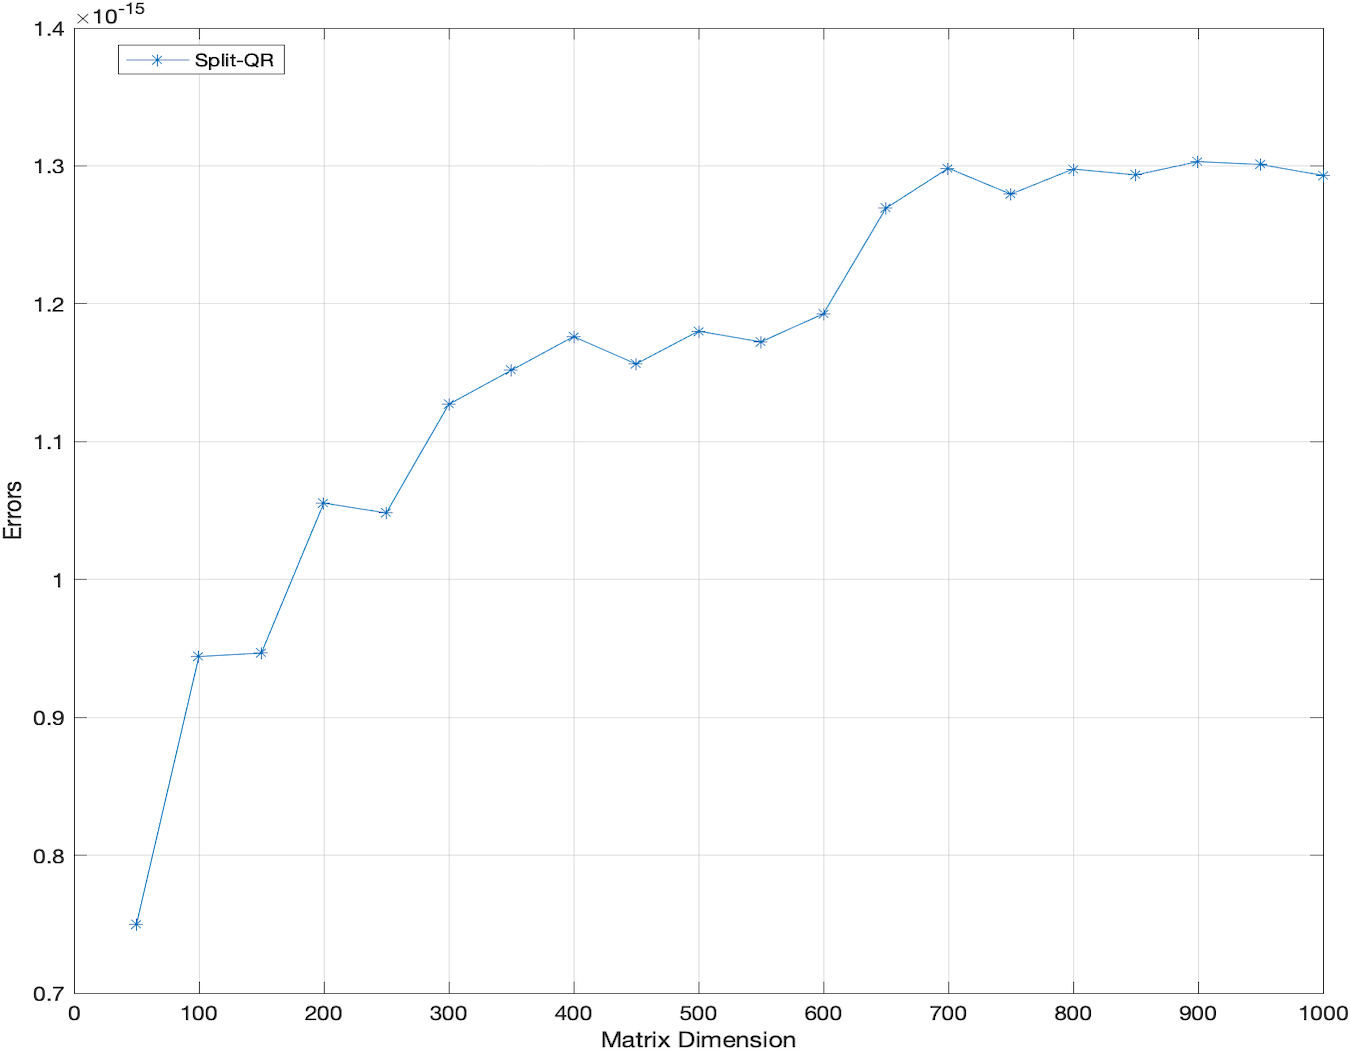
\includegraphics[width=0.45\textwidth]{images/Figure_3.png} % Replace with actual figure
    \caption{CPU Time (left) and Relative Error (right)}
  \end{figure}
  
  \begin{block}{Key Results}
    - CPU time scales linearly with $mn^2$ (matches complexity analysis)
    - Relative error $\epsilon \approx 10^{-15}$ (machine precision level)
  \end{block}
\end{frame}

\begin{frame}{5.2 Example 4.2: Application to Matrix Equation $AX = B$}
  \begin{block}{Problem Setup}
    Given $A,B \in \mathbb{H}_s^{3 \times 3}$ (explicit matrices in the paper), solve for $X \in \mathbb{H}_s^{3 \times 3}$.
  \end{block}
  
  \begin{block}{Solution Steps}
    1. Compute QR decomposition of $A$ via Algorithm 3: $A = QR$\\
    2. Multiply both sides by $Q^H$ (left): $RX = Q^H B \triangleq \hat{B}$\\
    3. Solve upper triangular system $RX = \hat{B}$ via back substitution
  \end{block}
  
  \begin{block}{Result}
    - Explicit $X$ constructed (see paper for details)\\
    - Relative error: $\frac{\|AX - B\|_F}{\|B\|_F} = 1.2412 \times 10^{-15}$ (high accuracy)
  \end{block}
\end{frame}

% Section 6: Conclusion
\section{6. Conclusion \& Future Work}
\begin{frame}{Outline}
  \tableofcontents[sectionstyle=show/shaded, subsectionstyle=show/show/shaded]
\end{frame}

\begin{frame}{6.1 Main Contributions}
  \begin{block}{Theoretical Contributions}
    1. Established the relationship $R_4 = P_{2m} R P_{2n}^T$ via permutations\\
    2. Proved existence of QR decomposition for split quaternion matrices (Theorem 3.1)\\
    3. Filled the gap in split quaternion QR decomposition theory
  \end{block}
  
  \begin{block}{Algorithmic Contributions}
    1. Proposed optimized permutation algorithm (Algorithm 2) to reduce computational cost\\
    2. Developed efficient Split-QR algorithm (Algorithm 3) with complexity $O(mn^2)$\\
    3. Validated high efficiency (speed) and accuracy via experiments
  \end{block}
\end{frame}

\begin{frame}{6.2 Future Work}
  \begin{block}{Extensions of the Real Representation Method}
    Apply the same framework to other decompositions:
    \begin{itemize}
      \item Schur decomposition
      \item Eigenvalue decomposition
      \item Generalized QR decomposition
    \end{itemize}
  \end{block}
  
  \begin{block}{Application Expansion}
    - Solve more complex split quaternion matrix equations (e.g., $AX + XB = C$)\\
    - Apply to real-world problems: Electromagnetic field simulation, quantum state estimation
  \end{block}
  
  \begin{block}{Data Availability}
    Data available upon request to the corresponding author (xiliu@must.edu.mo)
  \end{block}
\end{frame}

% References Page
\begin{frame}{References}
  \small
  \begin{thebibliography}{9}
    \bibitem{cockle1849} Cockle J (1849) On systems of algebra involving more than one imaginary. Phil. Mag. 35:434–437
    \bibitem{jiang2018} Jiang TS et al (2018) Eigenvalues of split quaternion matrices. Comput. Phys. Comm. 229:1–7
    \bibitem{wang2024} Wang G et al (2024) SVD for split quaternion matrices. J. Comput. Appl. Math. 436:115447
    \bibitem{si2024} Si KW et al (2024) A classical system of matrix equations over $\mathbb{H}_s$. Adv. Appl. Clifford Algebras 34:51
    \bibitem{liu2025} Liu Q et al (2025) An algorithm for QR decomposition of split quaternion matrices. (Submitted)
  \end{thebibliography}
\end{frame}



\logo{}

\begin{frame}
    \centering
    \vspace{1em}
    \Huge \textbf{Thank You!} \\
    \vspace{1.5em}
    \LARGE Questions and Discussion \\
    \vspace{2em}
    \begin{columns}[c]
        \column{0.3\textwidth}
        \centering
        
\includegraphics[height=1.2cm]{images/must-logo.png}
        
        \column{0.7\textwidth}
        \begin{flushleft}
            \large
            \textbf{Liu Qianqian} \\
            Faculty of Innovation Engineering \\
            Macau University of Science and Technology \\
            \faEnvelopeO \href{mailto:3240005215@student.must.edu.mo}{\texttt{\ 3240005215@student.must.edu.mo}}
        \end{flushleft}
    \end{columns}
\end{frame}

\end{document}